\newcommand{\bh}{\mathbf{h}} 
\newcommand{\bt}{\mathbf{t}} 
\newcommand{\bu}{\mathbf{u}} 
\newcommand{\bv}{\mathbf{v}} 
\newcommand{\bw}{\mathbf{w}} 
\newcommand{\bx}{\mathbf{x}} 
\newcommand{\bz}{\mathbf{z}} 
\newcommand{\by}{\mathbf{y}} 

\newcommand{\bA}{\mathbf{A}} 
\newcommand{\bC}{\mathbf{C}} 
\newcommand{\bI}{\mathbf{I}} 
\newcommand{\bT}{\mathbf{T}} 
\newcommand{\bW}{\mathbf{W}} 
\newcommand{\bX}{\mathbf{X}} 
\newcommand{\bZ}{\mathbf{Z}} 

\newcommand{\bepsilon}{\boldsymbol{\epsilon}}
\newcommand{\bmu}{\boldsymbol{\mu}}
\newcommand{\blambda}{\boldsymbol{\lambda}}
\newcommand{\bsigma}{\boldsymbol{\sigma}}
\newcommand{\bSigma}{\boldsymbol{\Sigma}}

\newcommand{\bbE}{\mathbb{E}} 
\newcommand{\bbP}{\mathbb{P}} 
\newcommand{\bbQ}{\mathbb{Q}} 
\newcommand{\bbR}{\mathbb{R}} 

\newcommand{\mbbP}{\mathbb{P}_{\text{MCMC}}}

\newcommand{\cL}{\mathcal{L}} 
\newcommand{\cN}{\mathcal{N}} 
\newcommand{\cS}{\mathcal{S}} 
\newcommand{\cT}{\mathcal{T}} 
\newcommand{\cX}{\mathcal{X}} 
\newcommand{\cB}{\mathcal{B}}
\newcommand{\cY}{\mathcal{Y}}
\newcommand{\cP}{\mathcal{P}}
\newcommand{\cF}{\mathcal{F}}
\newcommand{\cW}{\mathcal{W}}
\newcommand{\cE}{\mathcal{E}}
\newcommand{\cU}{\mathcal{U}}
\newcommand{\cV}{\mathcal{V}}
\newcommand{\cM}{\mathcal{M}} 

\newcommand\footfullcitenonum[1]{%
  \begingroup
  \renewcommand\thefootnote{}\footfullcite{#1}%
  \addtocounter{footnote}{-1}%
  \endgroup
}

\newcommand\footnotenonum[1]{%
  \begingroup
  \renewcommand\thefootnote{}\footnote{#1}%
  \addtocounter{footnote}{-1}%
  \endgroup
}

\definecolor{mgreen}{RGB}{0, 170, 0}

\newcommand{\green}[1]{{\color{mgreen} #1}}
\newcommand{\red}[1]{{\color{red} #1}}
\definecolor{myellow}{RGB}{255, 204, 0}
\newcommand{\yellow}[1]{{\color{myellow} #1}}

\definecolor{mysunset}{RGB}{255, 143, 1}
\newcommand{\sunset}[1]{{\color{mysunset} #1}}

\definecolor{mytwilight}{RGB}{29, 55, 176}
\newcommand{\twilight}[1]{{\color{mytwilight} #1}}

\newcommand{\bbRn}{\mathbb{R}^n}
% \newcommand{\bbR}{\mathbb{R}}
% \newcommand{\bbP}{\mathbb{P}} 

\section{Introduction}

В некоторых практических приложениях исследуемые данные лежат на на некотором многообразии $\cM^n \cong \bbR^n$ вложенного в $\bbR^N$, $n < N$. Необходимо построить модель машинного обучения, способную семлировать данные из целевого распределения/оценивать плотность целевого распределения. В качестве моделей рассматриваются потоковые структуры (то есть модели, обучающиеся с помощью метода максимизации правдоподобия и, как правило, обратимые)

\begin{figure}[!h]
\vspace{-5mm}
	    \centering
	  \vspace{2mm}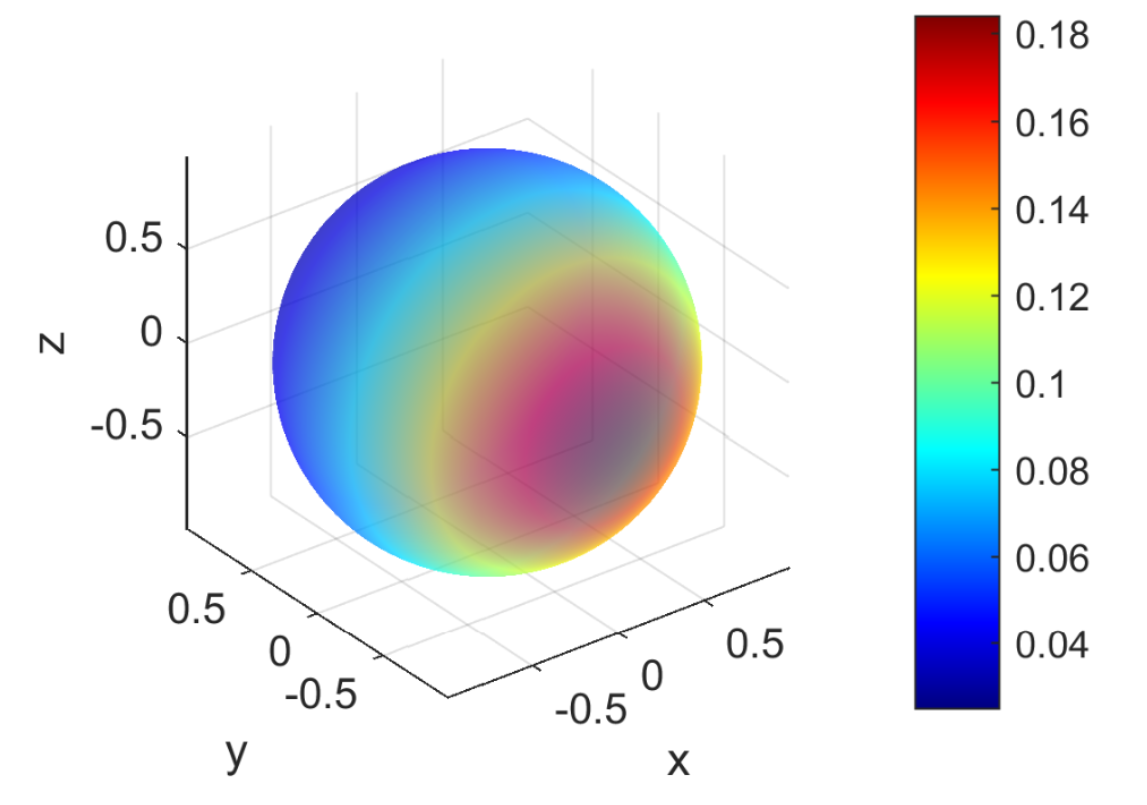
\includegraphics[width=0.5\linewidth]{chapters/petr_mokrov_s1/figs/VonMisesSphere.png}
	    \caption{{Пример von Mises-Fisher распр. на $S^2$}}
\end{figure}

\section{References Review}
\begin{itemize}
    \item \cite{dinh2017density} : В этой статье предлагается RealNVP - классическая Normalizing Flow модель.
    
    \item \cite{gemici2016normalizing} : Normalizing flows на многообразии, в предположении, что многообразие (карта) известна.
    
    \item \cite{beitler2019pie} : В этой статье предлагается PIE (Pseudo-Invertible Encoder) - одна из первых моделей, которая может учит многообразие и распределение на нём.
    
    \item \cite{NEURIPS2020_05192834} : Основная статья доклада, в ней предлагается $\cM$ и $\cM_e$ - потоки, явно учат целевое многообразие и честно оценивают плотность на нём, обучение двухстадийное (чередуются обучение карты и максимизация правдоподобия) что позволяет избежать оценки сложновычислимого якобиана карты.
    
    \item \cite{caterini2021rectangular} : Современный подход для обучения Rectangular flows на многообразии, при обучении с помощью различных технических процедур удаётся оценивать якобиан карты и производить оптимизацию исключительно максимизируя правдоподобие
\end{itemize}

\section{Main Part}

\subsection{Normalizing flows}

Напомним устройство классических нормализующих потоков. Имеется $x$ - целевая случайная величина, для латентной переменной $z$ фиксируется распределение. Строится $f: \bbR^N \rightarrow \bbR^N$ - диффеоморфизм. Формулы замены переменной: $p(x) = p(z) \left|\text{det}\left(\frac{\partial f(x, \theta )}{\partial x}\right)\right|$. Обучение производится с помощью MLE: 
 \vspace{-2mm}$$\arg\max\limits_{\theta \in \Theta} \sum\limits_i \log(p(f(x_i, \theta)) \log \left| \left(\frac{\partial f(x_i, \theta )}{\partial x_i}\right)\right|$$
 \vspace{-5mm}
 \begin{figure}[h]
    \centering
    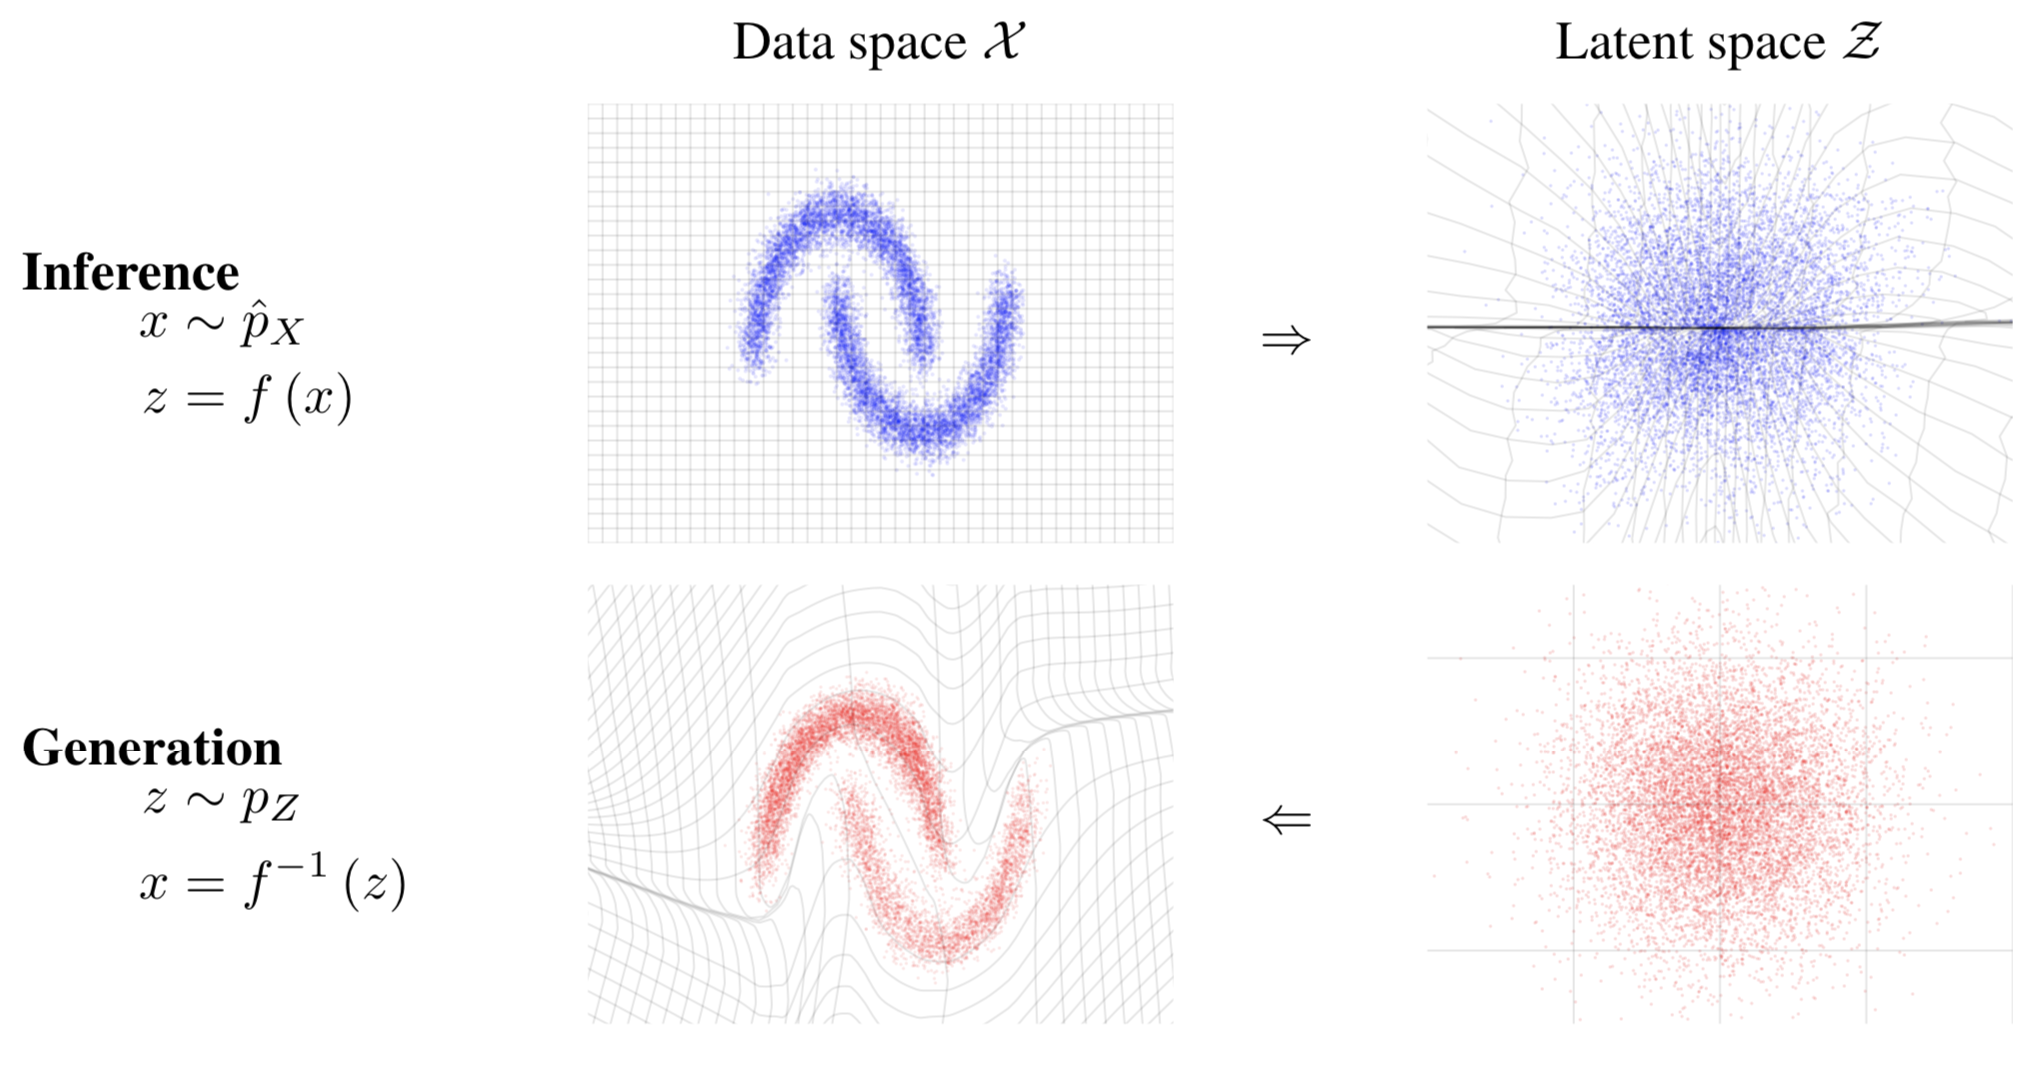
\includegraphics[width=0.5\linewidth]{chapters/petr_mokrov_s1/figs/flows_how2.png}
\end{figure}

При моделировании данных на многообразии классические нормализующие потоки обладают следующими недостатками: 
\begin{itemize}
    \item Распределение "размазанно" в окрестности целевого многообразия
    \item Вероятностная масса распределена в окрестности многообразия $\Rightarrow$ NF не моделирует истинную плотность
\end{itemize}
\begin{figure}[h]
    \centering
    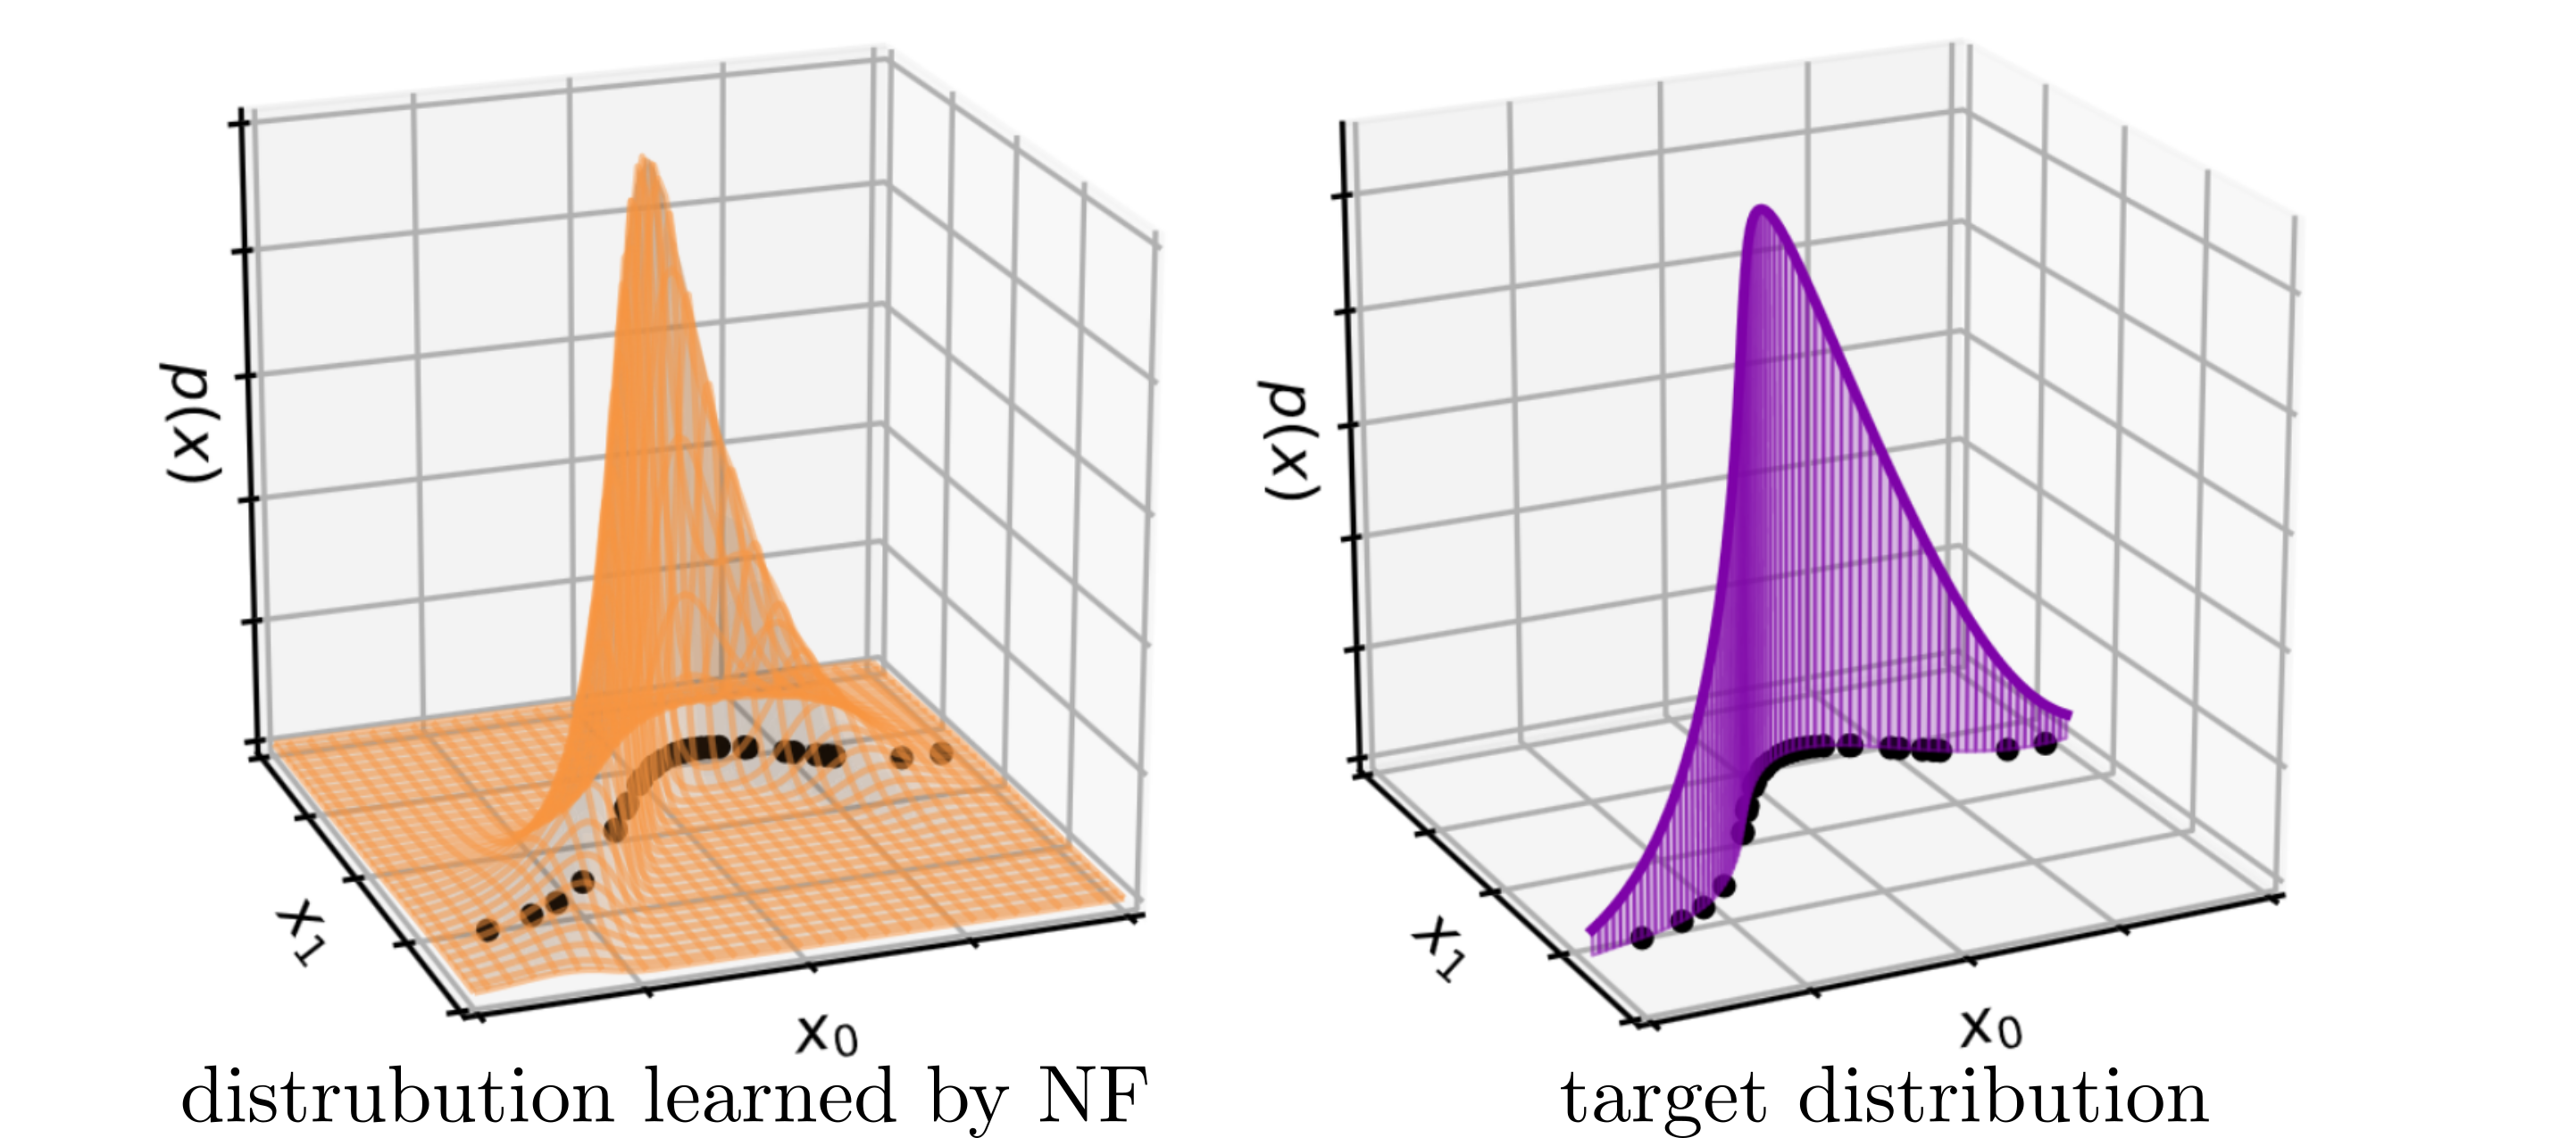
\includegraphics[width=0.6\linewidth]{chapters/petr_mokrov_s1/figs/nf_on_manifold_with_text.png}
\end{figure}

\newpage

\subsection{Notations}

Введём следующие обозначения: 

\begin{figure}[h]
    \centering
    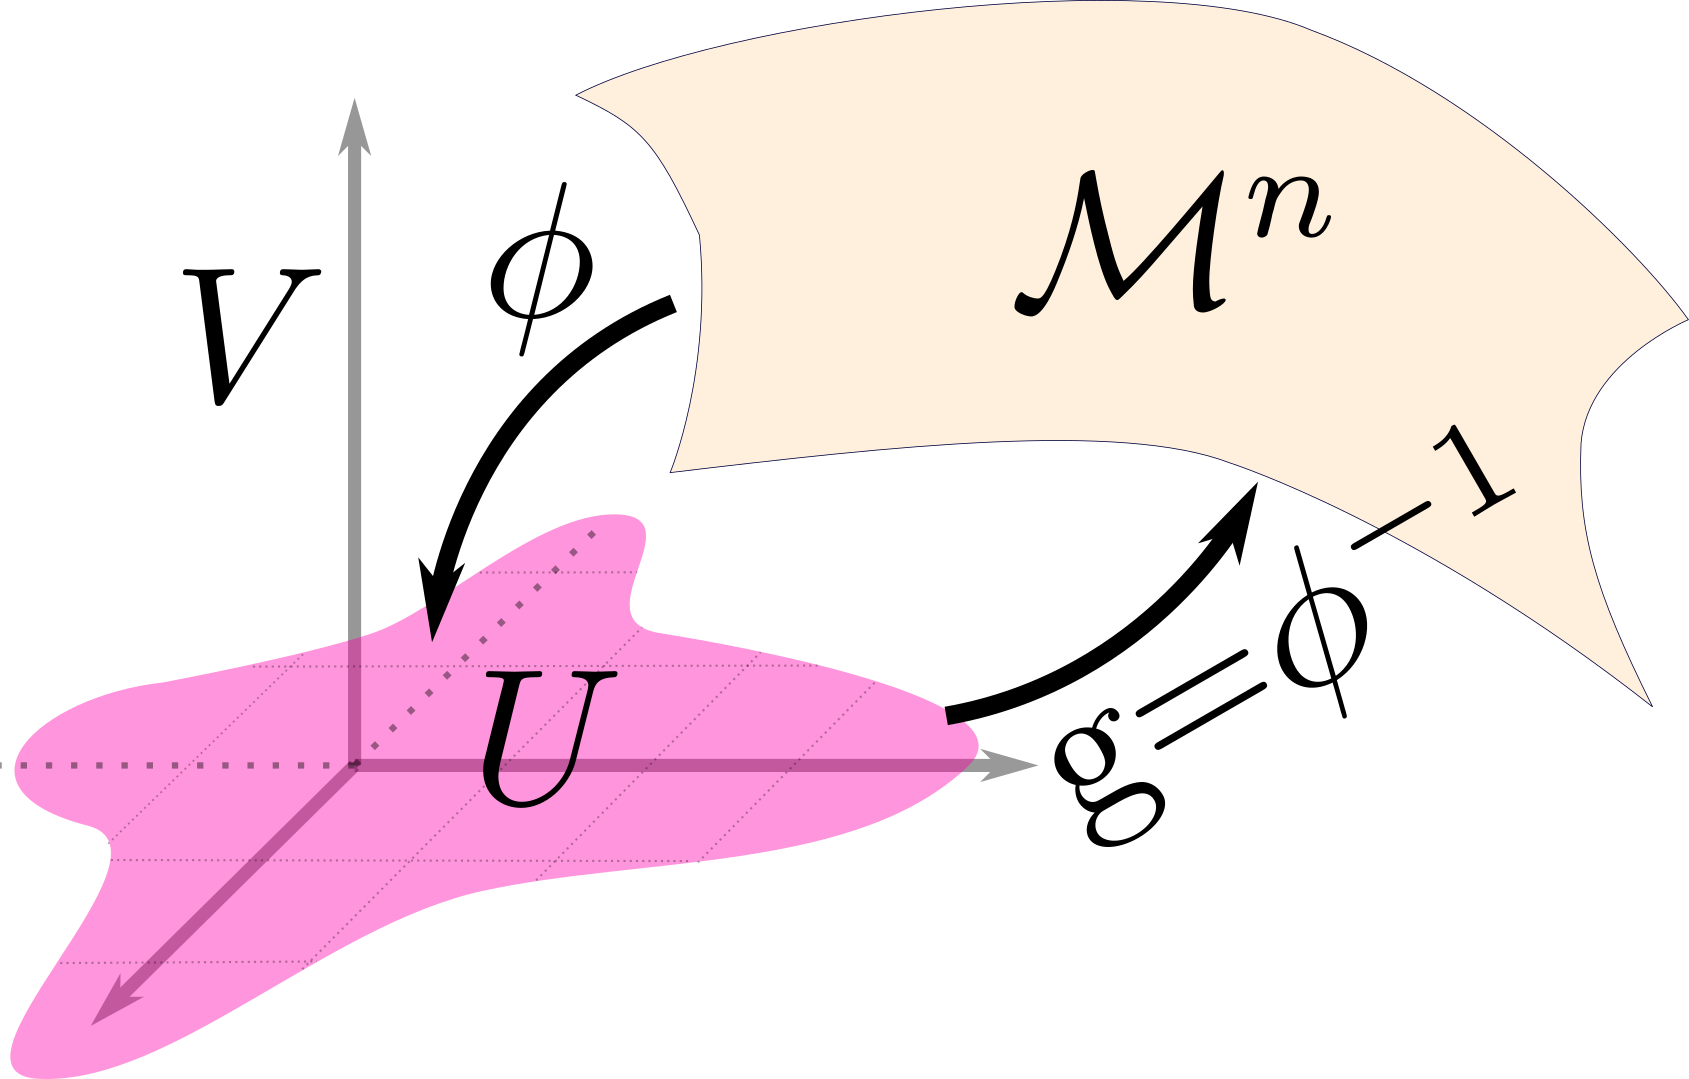
\includegraphics[width=0.4\linewidth]{chapters/petr_mokrov_s1/figs/notations4.png}
\end{figure}

\textbf{Manifold coordinates} В качестве $u \in U = \bbR^n$ мы будем обозначать вектора, которые отображаются в целевое многообразие $\cM^n$

\textbf{Off-the manifold coordinates} (остаточные координаты) В качестве $v \in V = \bbR^{N - n}$ мы будем обозначать оставшиеся координаты

\subsection{Flow on a manifold (FOM)}

В данном методе предполагается, что нам дано само многообразие и (обратная) карта: $g: U \rightarrow \cM^n$. Тогда верно следующее:

\begin{itemize}
    \item Из дифференциальной геометрии следует, что плотность на многообразии дана следующей формулой: 
    \begin{gather*}
        p_{\cM^n}(x) = p_{u}(g^{-1}(x)) \left|\det \left[J_g^T(g^{-1}(x)) J_g(g^{-1}(x))\right]\right|^{\frac{1}{2}} 
    \end{gather*}
    \item $J_g$ - якобиан карты $g$, матрица размера $n \times N$
    \item Плотность $p_u(u)$ в пространстве $U$ можно моделировать с помощью NF $$h : \tilde{U} (= U) \rightarrow U$$ рассматривая в качестве начальной плотности известную $p_{\tilde{u}}(\tilde{u})$
\end{itemize}

\begin{figure}[h]
    \centering
    \hspace*{-5mm}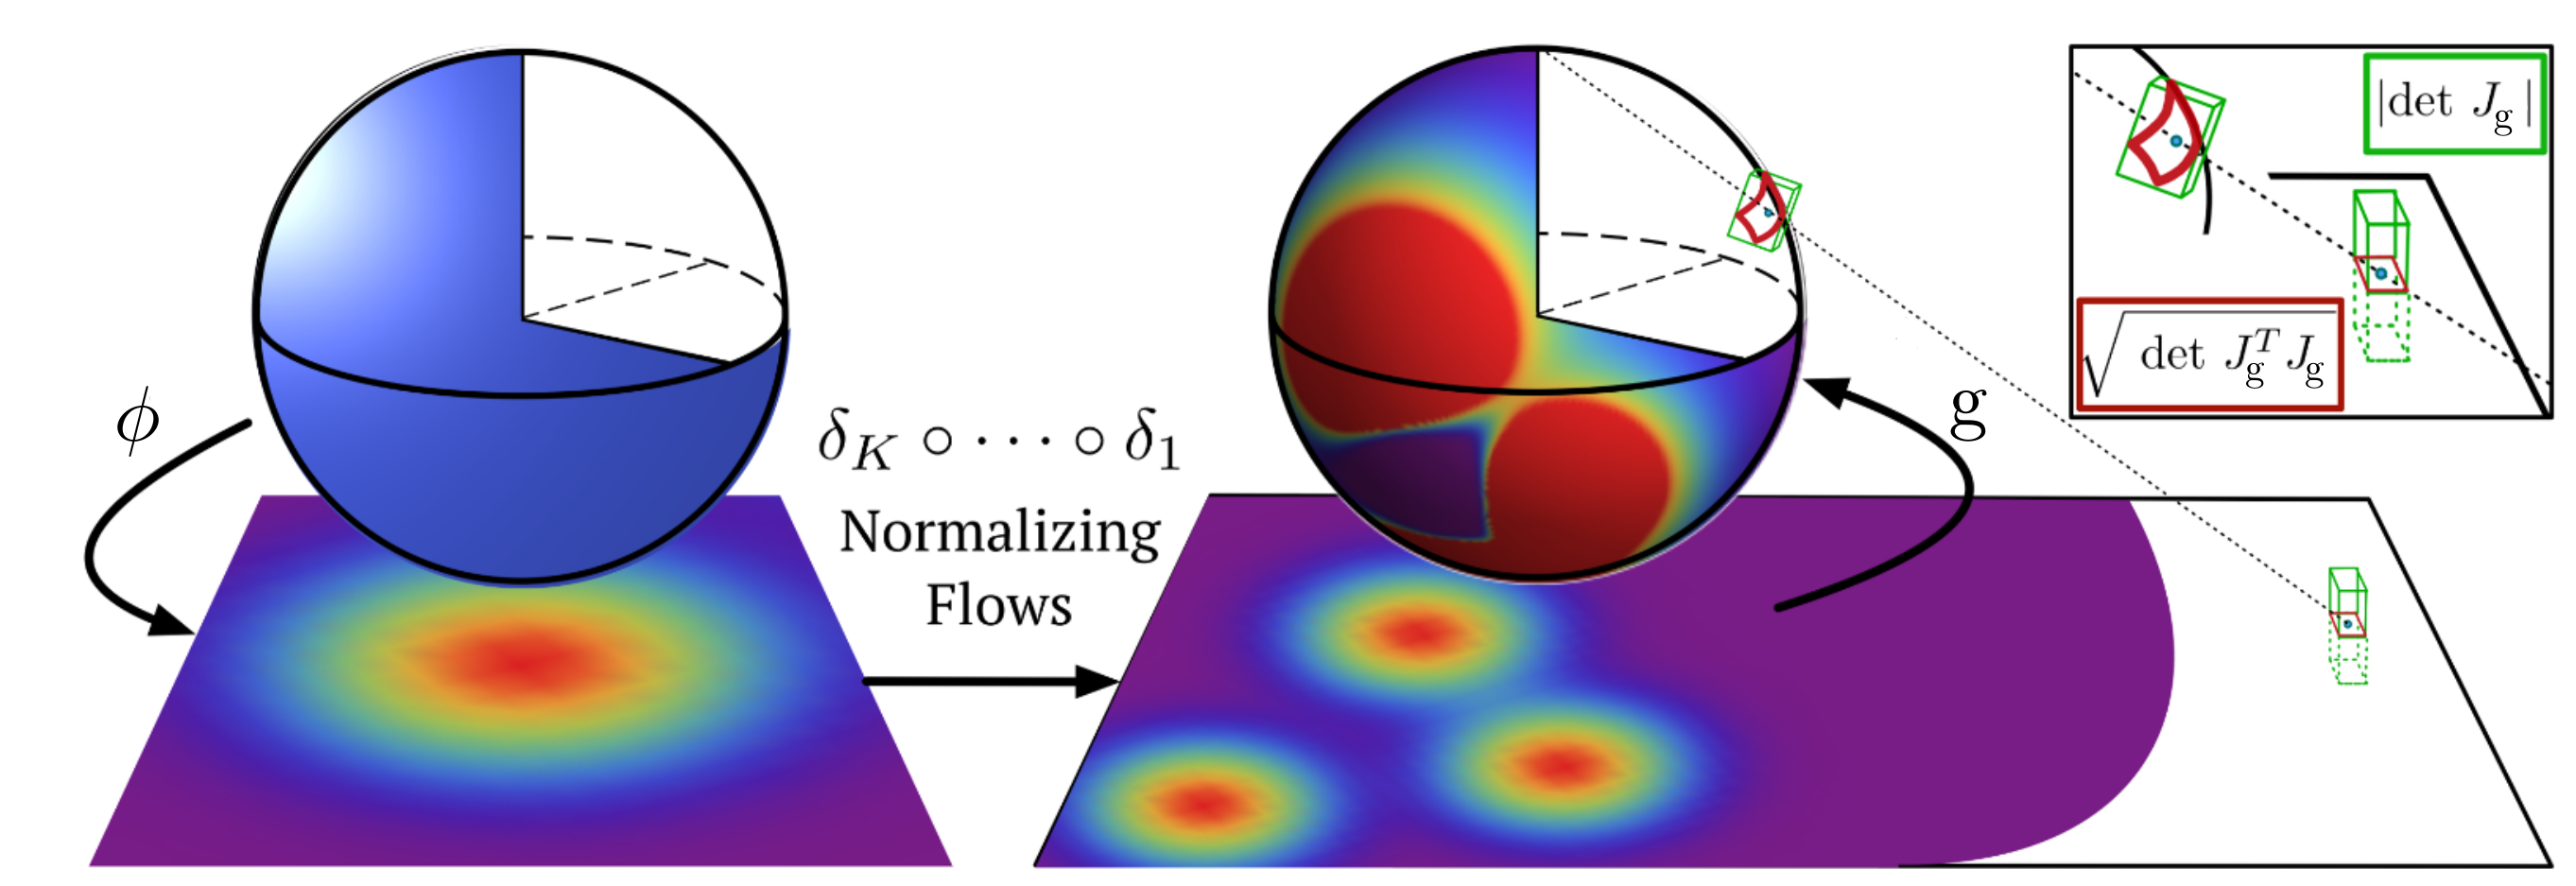
\includegraphics[width=0.7\linewidth]{chapters/petr_mokrov_s1/figs/fom_final.png}
\end{figure}

Достоинством данного подхода является возможность сведения задачи к классическим нормализующим потокам, важным недостатком явлется небоходимость знать карту целевого многообразия.

\newpage

\subsection{PIE: Pseudo-Invertible Encoder (V1)}

Одной из первых моделей, короая учит как плотность на многообразии, так и само многообразие, является PIE. 

\begin{figure}[h]
    \centering
    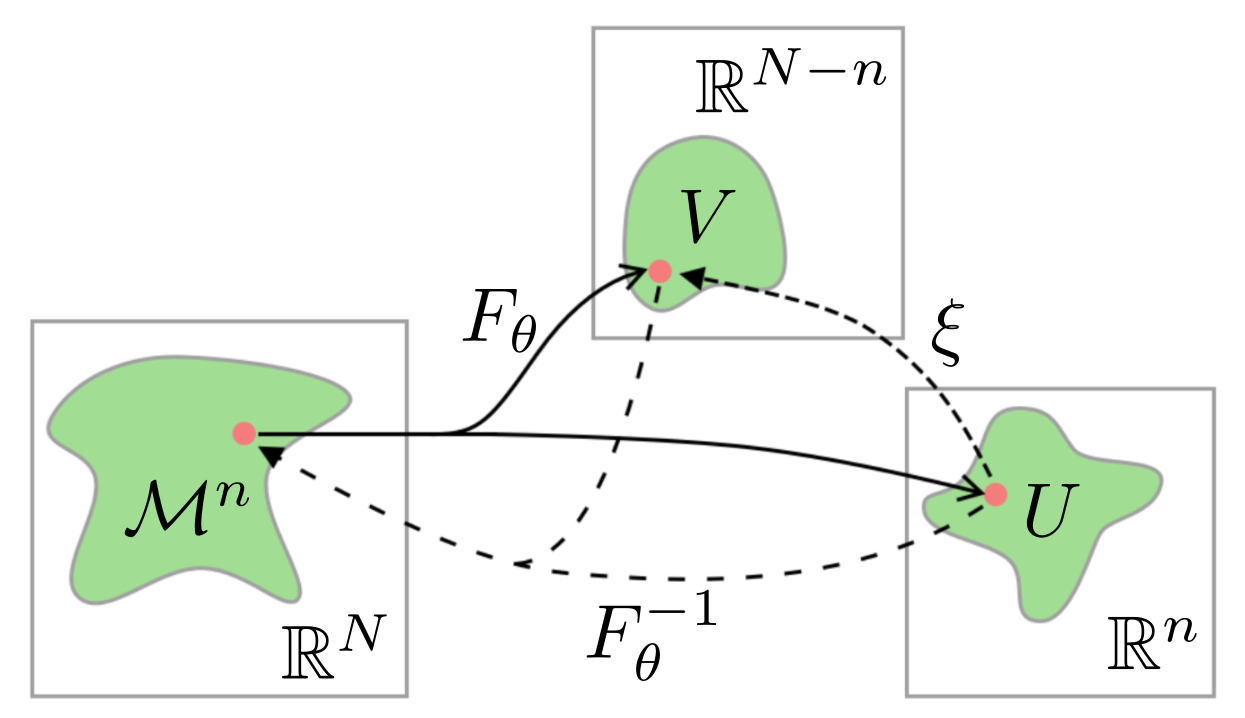
\includegraphics[width=0.5\linewidth]{chapters/petr_mokrov_s1/figs/pie_v1_final3.png}
\end{figure}

\begin{itemize}
    \item Модель по разному обрабатывает локальные координаты многообрзия $u \in U$ и остаточные координаты $v \in V$
    \item Вектор $v \in V$ генерируется из $u \in U$ с помощью фиксированной (или обучаемой) функции $\xi$
    \item Пара векторов $(u, v = \xi(u))$ преобразуется в точку на многообразии с помощью обучаемой модели $F_{\theta}^{-1}$ (поток $\bbR^N \rightarrow \bbR^N$)
\end{itemize}

На инференсе и при обучении модель работает следующим образом: 

\textbf{Genereative mode}
Для генерации семплируется $u \in U$, считается $v = \xi(u)$, преобразуется в целевую точку на многообразии $F_{\theta}^{-1}(u, \xi(u))$

\textbf{Log Likelihood}
Правдоподобие в точке на многообразии $x \in \cM^n$ оценивается так ($\epsilon_0$ - достаточно маленький): 
\vspace{-2mm}
\begin{gather*}
    \log p(x) = \log \det \left(J_{F_{\theta}}(x)\right) + \log p(u, v) \approx \\
    \approx \log \det \left(J_{F_{\theta}}(x)\right) + \log \cN(v | \xi(u), \epsilon_0 I) + \log p(z)
\end{gather*}

\green{Достоинства модели}: Модель учит целевое многообразие; обученная модель в generative mode семплирует из целевого многообразия

\red{Недостатки модели}: о построению нет критерия принадлежности точки многообразию; обучаемое распределение $p(x)$ не есть распределение на многообразии ($\log \det (J_{F_{\theta}}(x))$ - должно быть вырождено)

\newpage

\subsection{PIE: Pseudo-Invertible Encoder (V2)}

Была предложена модификация предыдущей модели, которая более явно разделяет обучение карты многообразия и плотности в пространстве координат: 

\begin{figure}[h]
    \centering
    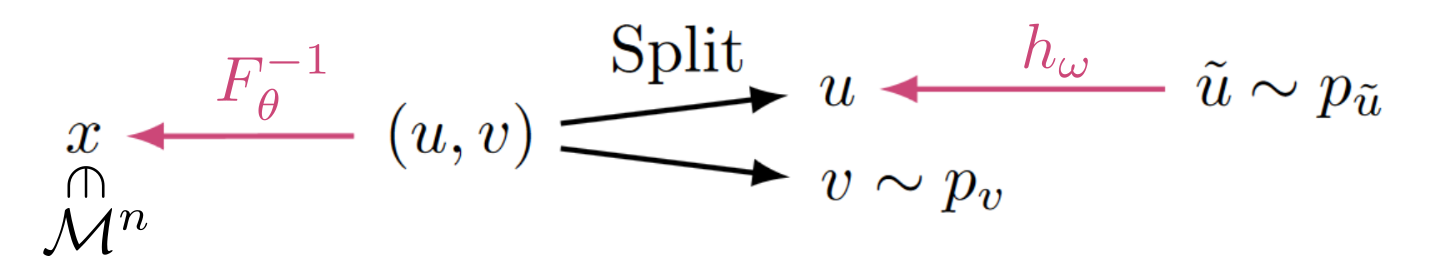
\includegraphics[width=0.6\linewidth]{chapters/petr_mokrov_s1/figs/pie_v2_final.png}
\end{figure}

Модель обладает следующими свойствами: 
\begin{itemize}
    \item Выбор функции $\xi$ не столь важен, берём $\xi = 0$
    \item Распределением $p_v$ служит $\cN(0, \epsilon_0 I)$
    \item Добавляем дополнительное отображение $h_{\omega}$ (поток $\bbR^n \rightarrow \bbR^n$), модифицирующее базовую плотность $p_{\tilde{u}}$ в пространстве координат
    \item \textbf{Note}: Интуитивно, мы бы хотели, чтобы $h_{\omega}$ учило правильную плотность в пространстве координат, а $F_{\theta}$ учило бы истинную карту многообразия $\cM^n$ 
\end{itemize}

Модель обладает теми-же недостатками, что и предыдущая модель. Для того, чтобы их решить, были предложены $\cM$ и $\cM_e$ потоки

\subsection{$\cM$-flow}

Предложенна модель удовлетворяет следующей схеме:

\begin{figure}[h]
    \centering
    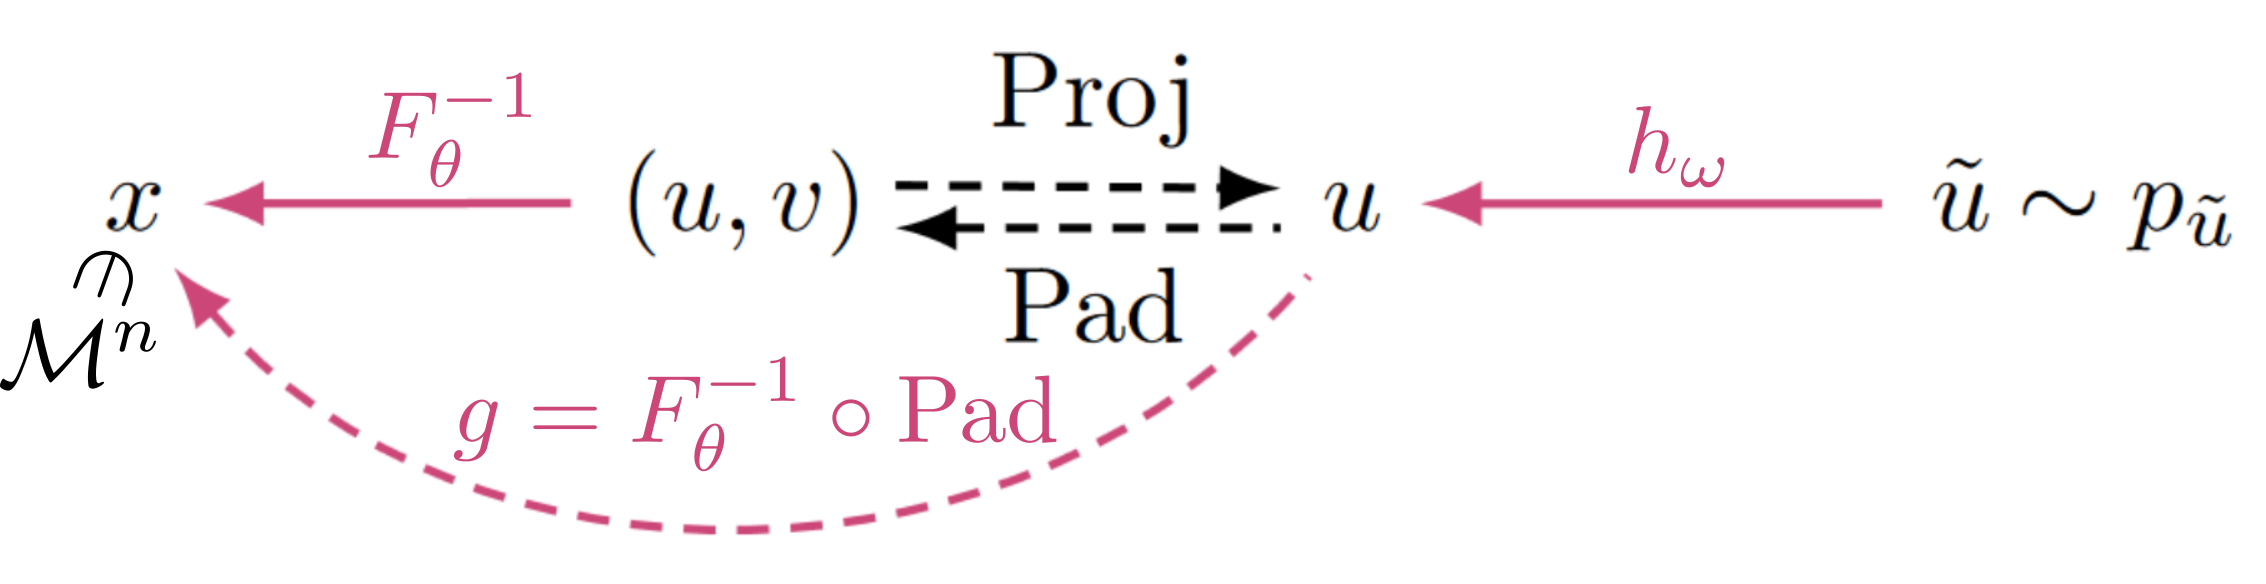
\includegraphics[width=0.6\linewidth]{chapters/petr_mokrov_s1/figs/mflow_final.png}
\end{figure}

Генерация и оценка правдоподобия делается следующим образом:

\textbf{Genereative mode}
Для генерации семплируется $u = h_{\omega}(\tilde{u}) \in U$, дополняется вектором $v = 0_{N - n}$ и преобразуется в целевую точку на многообразии $F_{\theta}^{-1}(u, 0_{N - n}))$

\textbf{Log Likelihood}
Правдоподобие в точке на многообразии $x \in \cM^n$:
\begin{gather*}
    \log p(x) = \log p_{\tilde{u}}(h_{\omega}^{-1}\circ g^{-1}(x)) - \log \det J_{h_{\omega}}(h_{\omega}^{-1}\circ g^{-1}(x)) - \\
    - 0.5 \log \det \left[ J_g^{T}(g^{-1}(x)) J_g(g^{-1}(x))\right]
    % \log \det \left(\frac{\partial F_{\theta}}{\partial x}\right) + \log p(u, v) \approx \\
    % \approx \log \det \left(\frac{\partial F_{\theta}}{\partial x}\right) + \log \cN(v | \xi(u), \epsilon_0 I) + \log p(z)
\end{gather*}

\subsubsection{Manifold chart learning}

Модель $\cM$ явным образом учит карту многообразия следующим образом: 
\begin{itemize}
    \item Поток $F_{\theta}$ в рамках всей модели учится представлять карту многобразия, для $x \in \cM^n$ минимизируемый лосс: 
    \vspace{-2mm}
    \begin{gather*}
        \cL_{\text{chart}} = \Vert x - g\left(\text{Proj}_{U}\left[F_{\theta}(x)\right]\right)\Vert
    \end{gather*}
    \item Имея $y \in \bbR^N$ карта $F_{\theta}$ определяет расстояние до многообразия: $\Vert y - g\left(\text{Proj}_{U}\left[F_{\theta}(y)\right]\right)\Vert$!
\end{itemize}

\begin{figure}[h]
    \centering
    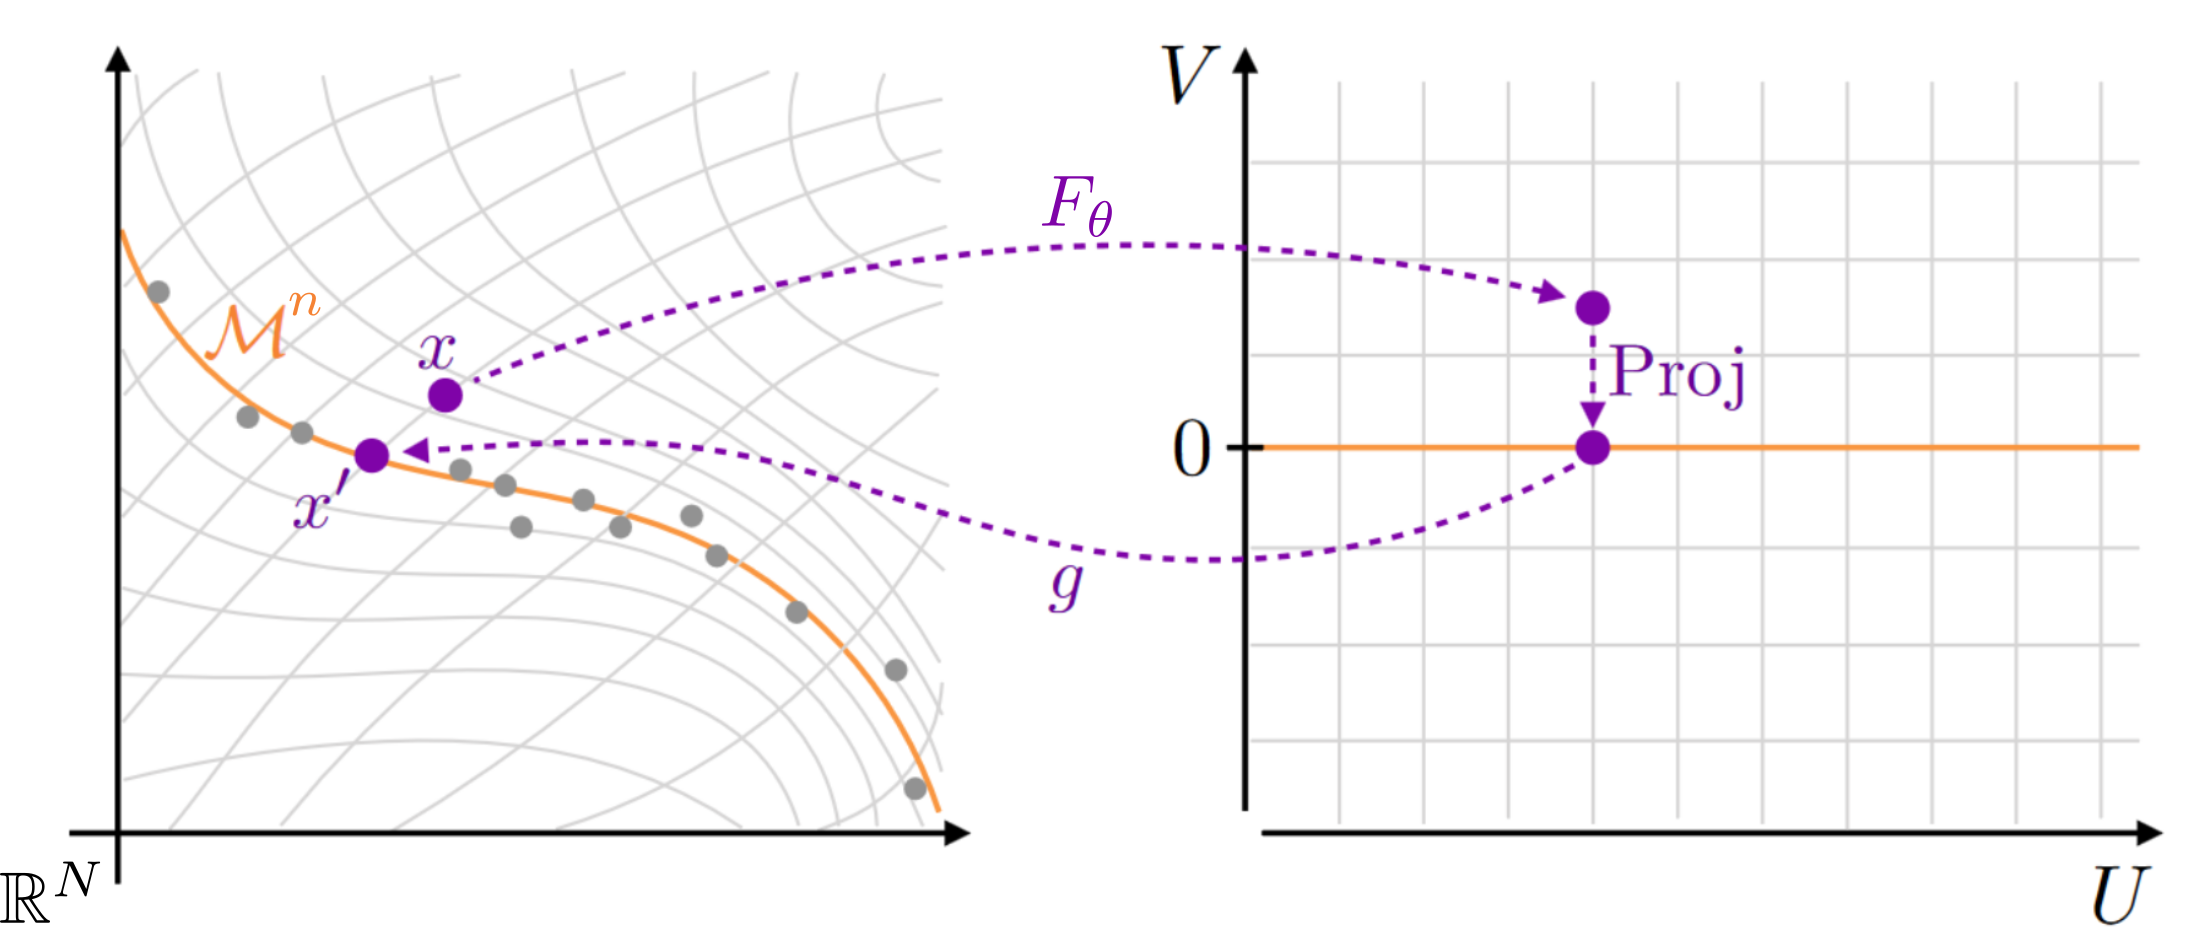
\includegraphics[width=0.6\linewidth]{chapters/petr_mokrov_s1/figs/mflow_manifold_final2.png}
\end{figure}

\subsubsection{Learning}

При обучении $cM$-потока чередуются два этапа: 
\begin{enumerate}
    \item Максимизация правдоподобия при фиксированной $F_{\theta}$
    \item Обучение карты $F_{\theta}$ при фиксированном распределении в пространстве координат $h_{\omega}\sharp p_{\tilde{u}}$ минимизируя лосс $\cL_{\text{chart}}$
\end{enumerate}

\subsection{$\cM_e$-flow}

Модифицированной версией $\cM$-потока является модель $\cM_e$-flow, представленная на схеме ниже: 

\begin{figure}[h]
    \centering
    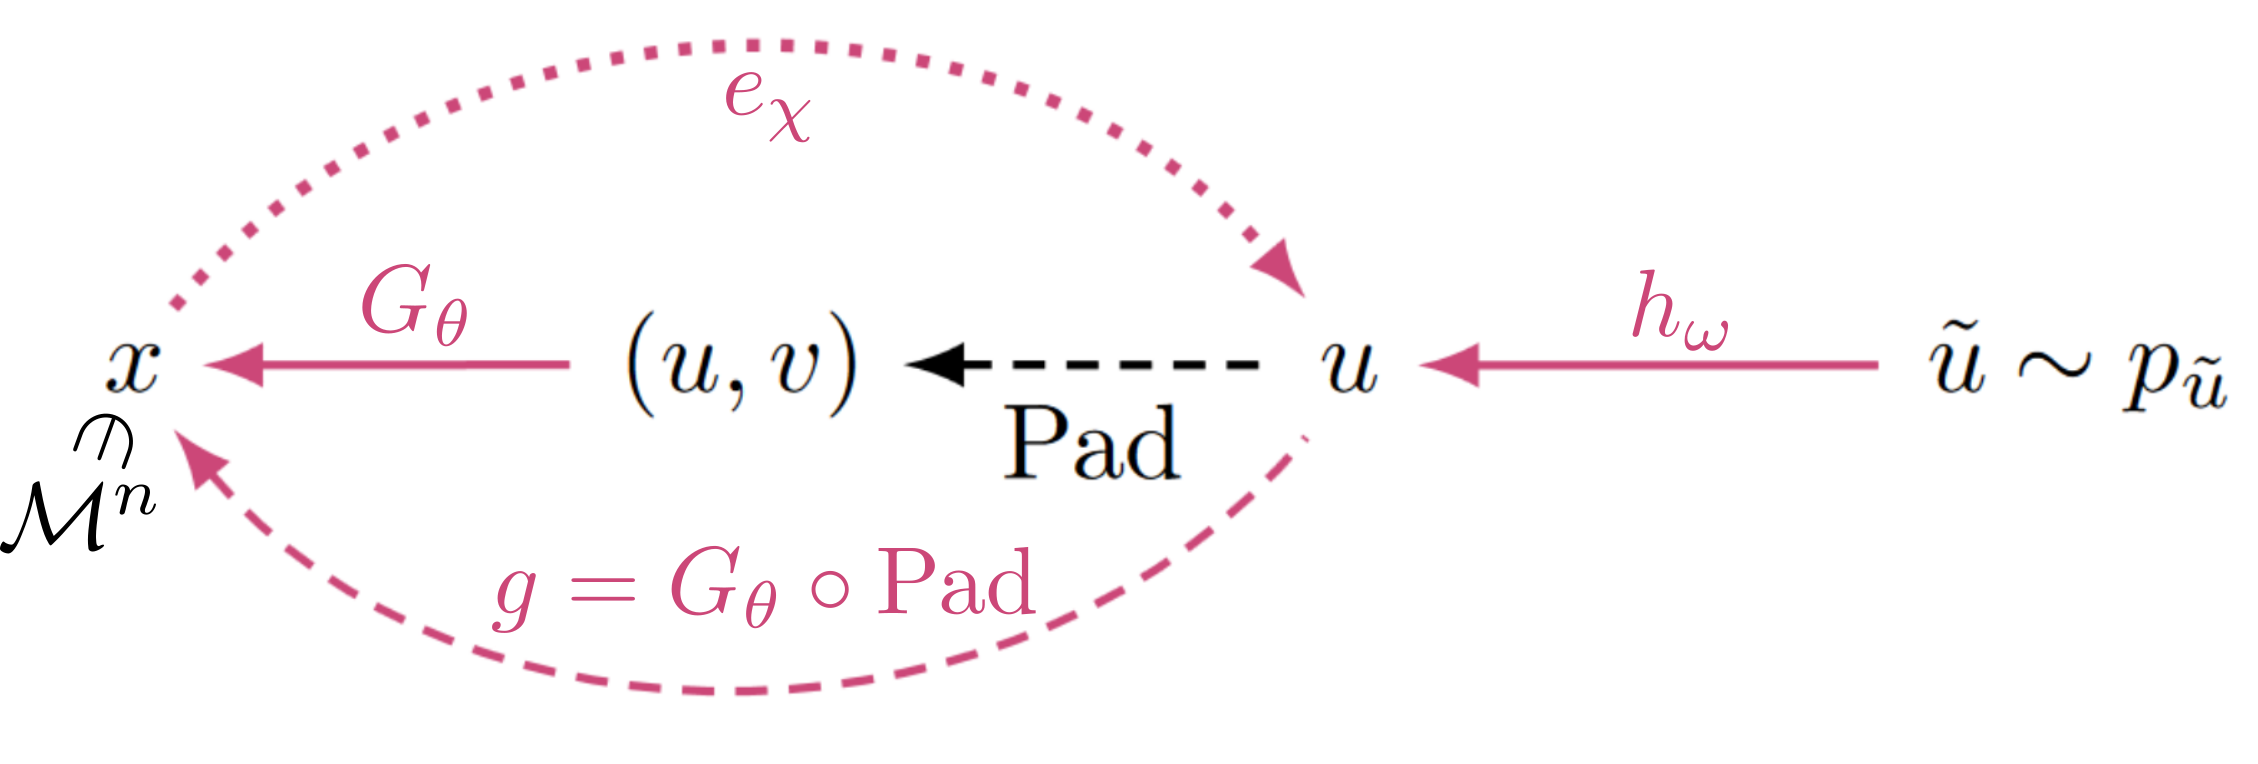
\includegraphics[width=0.6\linewidth]{chapters/petr_mokrov_s1/figs/mEflow_final.png}
\end{figure}

Особенности модели: 
\begin{itemize}
    \item Карта $g = G_{\theta} \circ \text{Pad}$ и (обратная) карта $e_{\chi}$ - разные модели
    \item $G_{\theta}$ и $e_{\chi}$ - не обязательно должны быть инвертируемы.
\end{itemize}

\newpage

\subsection{$\cM$ \& $\cM_{e}$-flows: Summary}

\textbf{\green{Достоинства модели}}
\begin{itemize}
    \item Модель явно учит карту многообразия $F_{\theta}$
    \item Естественным образом формулируется расстояние и проекция точки $y \in \bbR^N$ на многообразие $\cM^n$
    \item Легко оценивать отношение плотностей в байесовском инференсе (позднее!)
\end{itemize}
\textbf{\red{Недостатки модели}}
\begin{itemize}
    \item Вычисление плотности - \textbf{дорогое}, из-за необходимости вычисления якобиана карты: $\det \left[ J_g^{T}(g^{-1}(x)) J_g(g^{-1}(x))\right]^{\frac{1}{2}}$
    \item При раздельном обучении карты $F_{\theta}$ и плотности в пространсте координат $h_{\omega}$ карта может делать сжатия/растяжения, усложняющие обучение модели плотности.
\end{itemize}

В дальнейших секциях мы рассмотрим различные модельные задачи, а также приложения изученных моделей

\subsection{Test case: Gaussian on a Circle}

В даном эксперименте в качестве многообразия рассматривается круг, распределение на многообразии дано распределением на полярных угловых координатах $\theta \sim \cN(\pi/2, \pi/4)$

\begin{figure}[h]
    \centering
    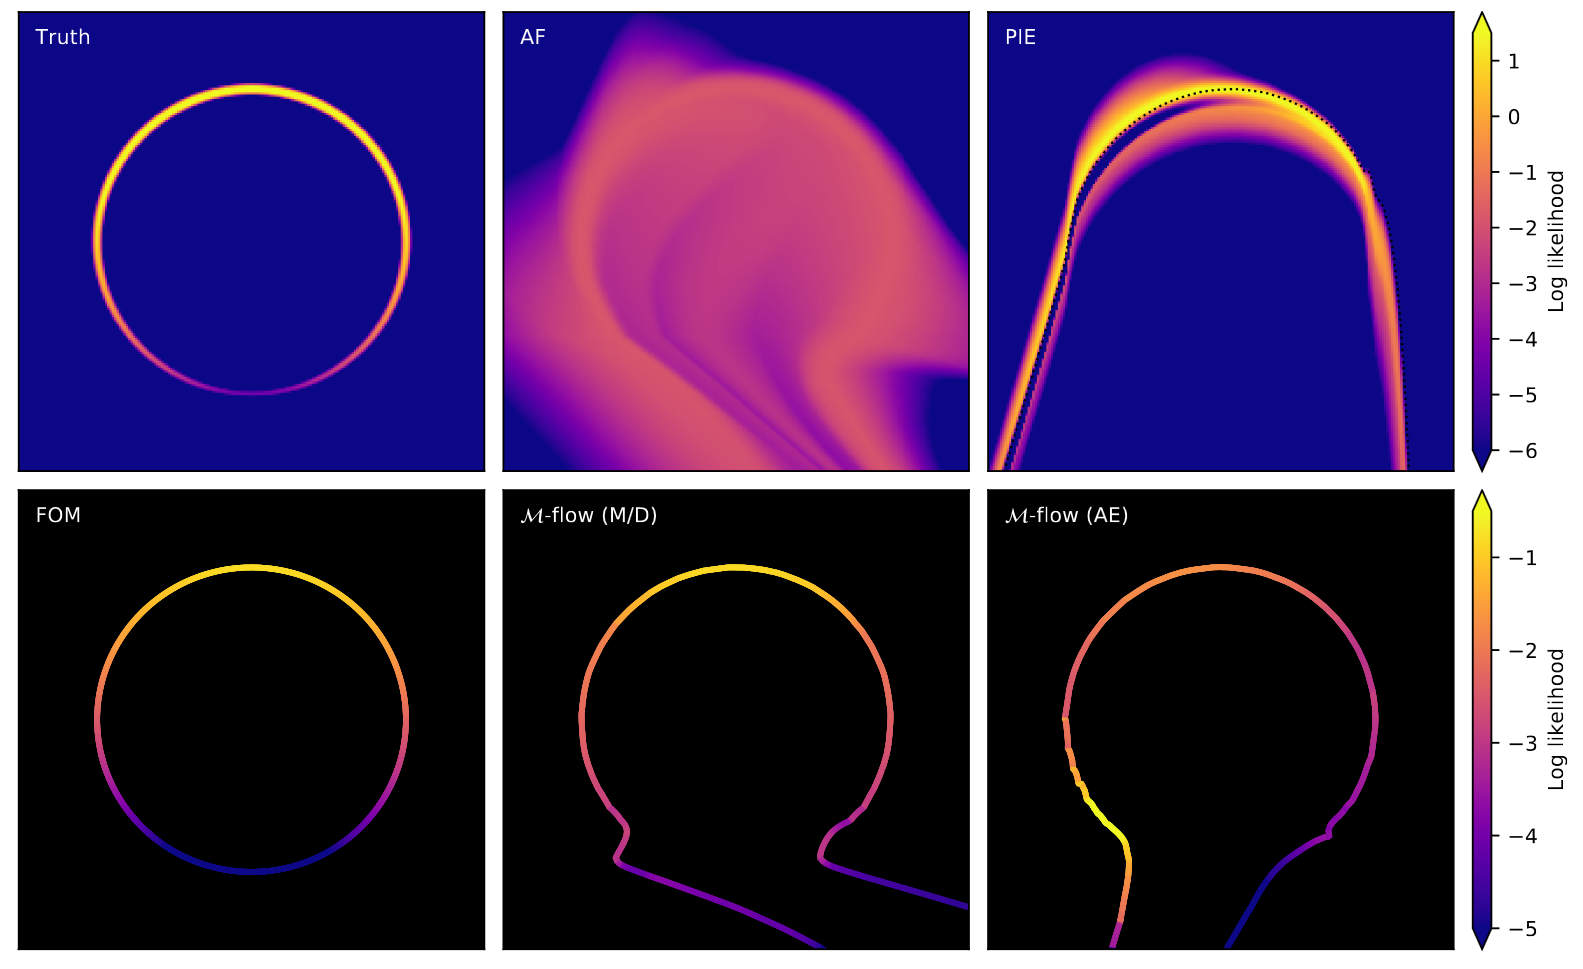
\includegraphics[width=0.7\linewidth]{chapters/petr_mokrov_s1/figs/gauss_in_circ.png}
\end{figure}

AF - классический нормализующий поток; Модель $\cM$-flow (AE) в отличие от $\cM$-flow (M/D) обучалась только правильно отражать координаты в многообразие.

\newpage

\subsection{Test case: Lorenz attractor}

Рассматривается Аттрактор Лоренца - Геометрическое Место траекторий дифференциального уравнения: 
\begin{gather*}
\begin{cases}
dx_0/dt = \sigma(x_1 - x_0) \\
dx_1/dt = x_0(\rho - x_2) - x_1\\
dx_2/dt = x_0 x_1 - \beta x_2
\end{cases}\\
\sigma=10, \beta = 8/3, \rho=28
\end{gather*}
% $\sigma=10, \beta = 8/3, \rho=28$

Аттрактор Лоренца образует многообразие размерности $\approx 2$. Для моделирования используются $\cM$-flows, обучаются на точках, равномерно распределённых на траекториях.

\begin{figure}[h]
    \centering
    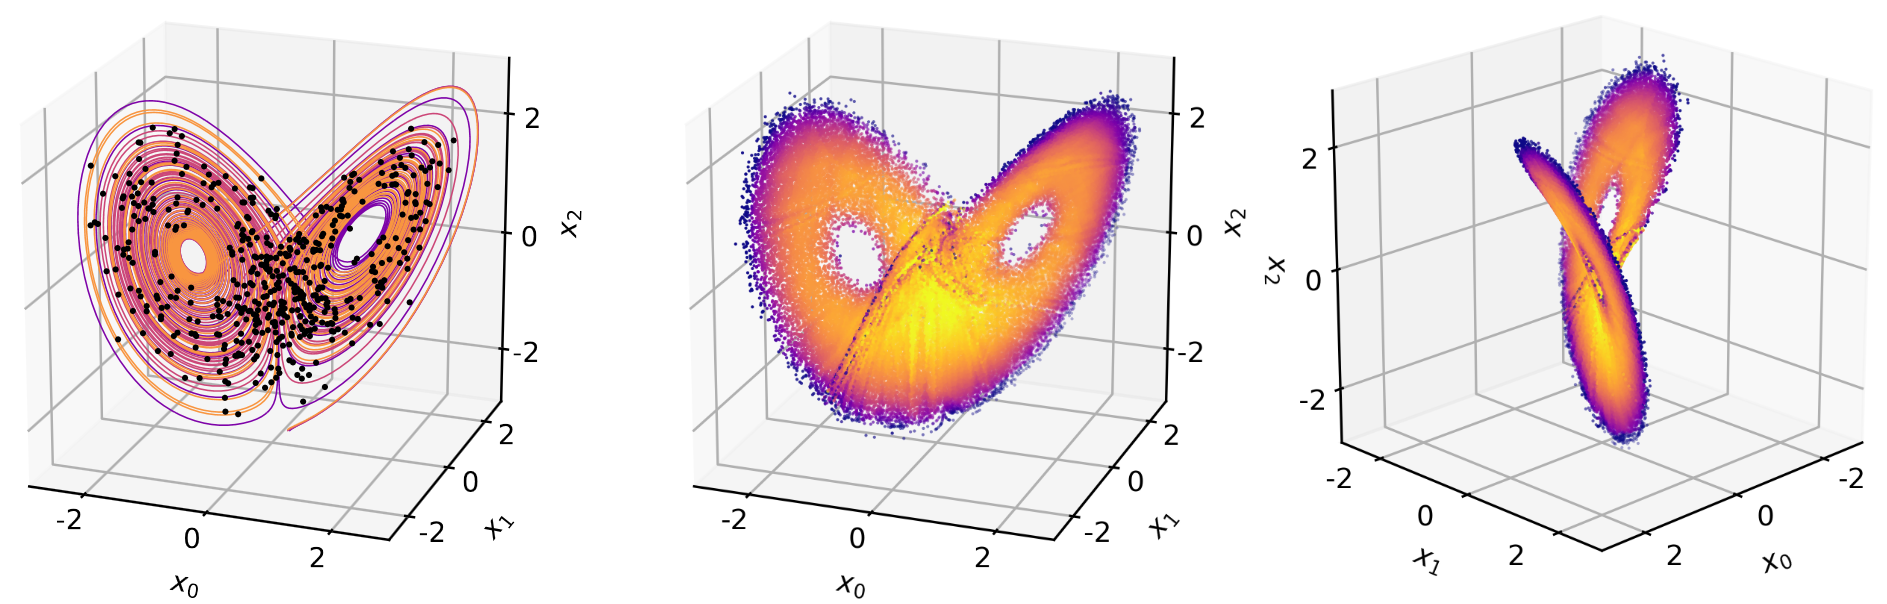
\includegraphics[width=0.7\linewidth]{chapters/petr_mokrov_s1/figs/lorenz_attractor.png}
\end{figure}

На левом рисунке изображены истинные траектории дифференциального уравнения с просемплированными точками. На правых двух рисунках изображено выученное многообразие.

\subsection{Likelihood-free simulation-based inference}

Рассмотрим задачу likelihood-free simulation-based inference. Данная задача формулируется следующим образом: 
\begin{itemize}
    \item Дан симулятор $p_{\text{model}}(x | \zeta)$, описывающая некоторую физическую реальность обусловленную на параметры модели/константы природы (плотность не дана!)
    \item Требуетcя вычислить апостериорную плотность (Bayesian inference):
    \vspace{-2mm}
    \begin{gather*}
        p(\zeta | X) = \frac{p(X | \zeta) p(\zeta)}{\int_{Z} d \zeta' p(X | \zeta') p(\zeta')}
    \end{gather*}
\end{itemize}

\newpage

На рисунке ниже изображены примеры симуляторов: слева показана модель, семплирующая картинку из MNIST по параметру - цифре. Справа схематически показана модель, расчитывающая какие-либо физические экспериментальные величины (спектры поглощения/излучения частиц, например) чёрной дырой по массе и угловой скорости чёрной дыры 

\begin{figure}[h]
    \centering
    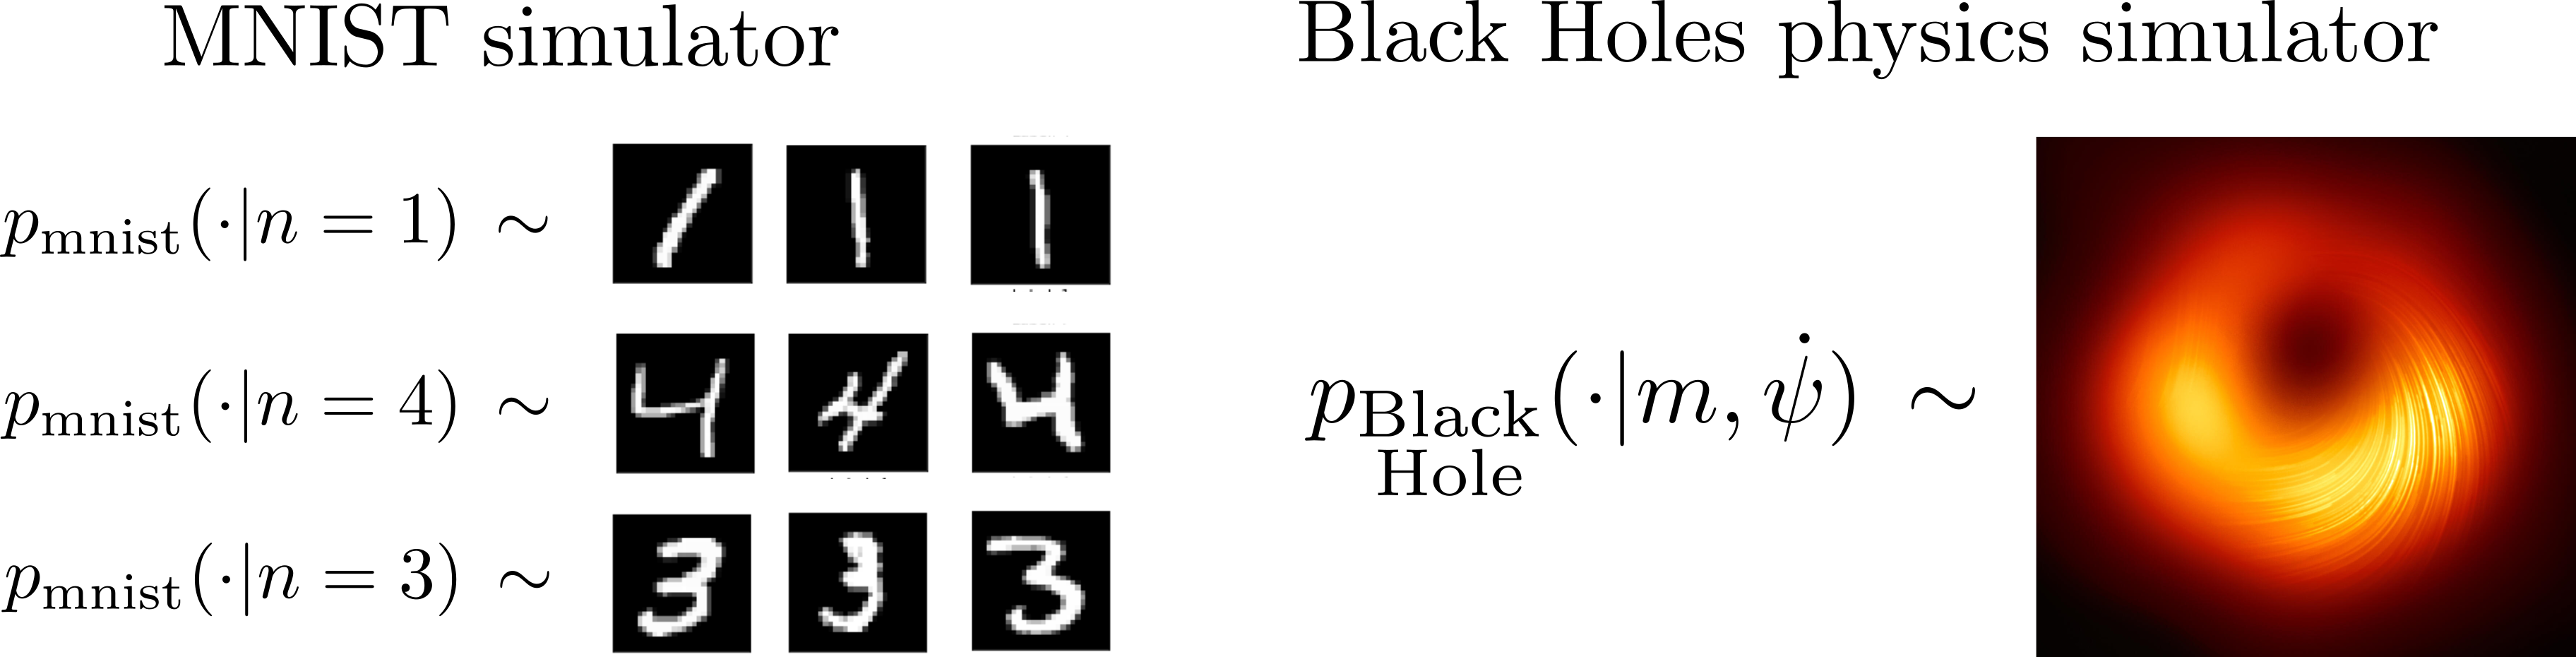
\includegraphics[width=0.7\linewidth]{chapters/petr_mokrov_s1/figs/simulators_demo.png}
\end{figure}

\subsubsection{$\cM$-flows for simulation-based inference}

Напомним схему $\cM$-потока: 
\begin{figure}[h]
    \centering
    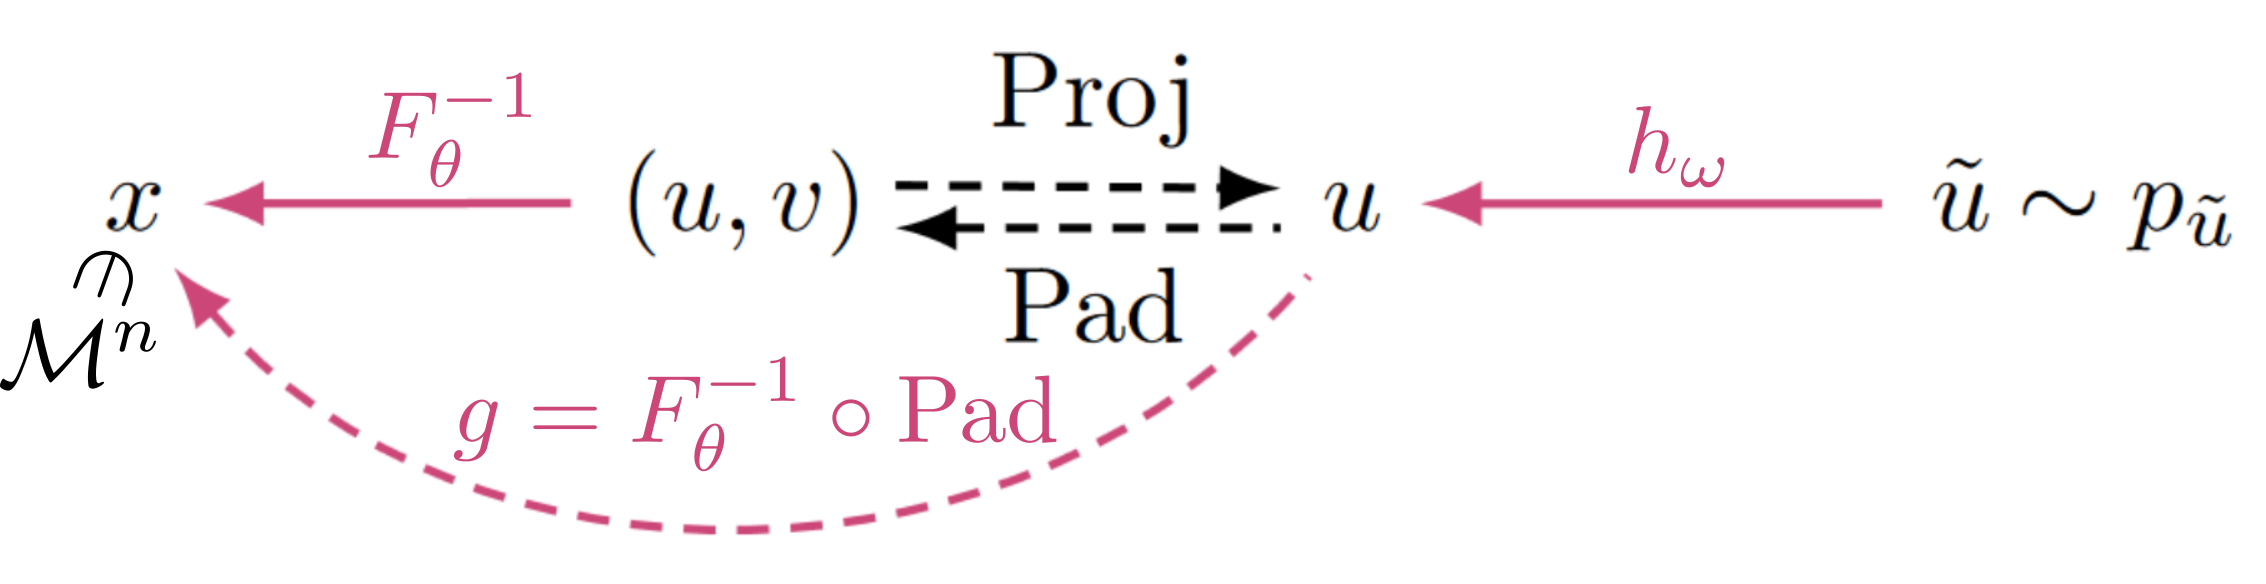
\includegraphics[width=0.6\linewidth]{chapters/petr_mokrov_s1/figs/mflow_final.png}
\end{figure}

Пусть многообразие $\cM^n$ \textbf{не зависит} от параметра $\zeta$. Тогда плотность на многообразии имеет следующий вид:
\begin{gather*}
    p(x| \zeta) = p_{\tilde{u}}(h_{\omega}^{-1}\left\{g^{-1}(x)| \zeta\right\}) \cdot \det J_{h_{\omega}}\left[h_{\omega}^{-1}\left\{g^{-1}(x)| \zeta\right\}\right]^{-1} \cdot \\ \cdot \det \left[ J_g^{T}(g^{-1}(x)) J_g(g^{-1}(x))\right]^{\frac{1}{2}}
\end{gather*}
При этом отношение плотностей при разных значениях параметра $\zeta$ не зависит от якобиана карты! ($\Rightarrow$ нам его не нужно вычислять):
\begin{gather*}
        \frac{p(x|\zeta_1)}{p(x|\zeta_2)} = \frac{p_{\tilde{u}}(h_{\omega}^{-1}\left\{g^{-1}(x)| \zeta_1\right\}) \cdot \det J_{h_{\omega}}\left[h_{\omega}^{-1}\left\{g^{-1}(x)| \zeta_1\right\}\right]^{-1}}{p_{\tilde{u}}(h_{\omega}^{-1}\left\{g^{-1}(x)| \zeta_2\right\}) \cdot \det J_{h_{\omega}}\left[h_{\omega}^{-1}\left\{g^{-1}(x)| \zeta_2\right\}\right]^{-1}}
\end{gather*}

\newpage

Это свойство можно использовать в алогоритме Метрополиса-Гастингса для MCMC семплирования из апостериорной плотности $p(\zeta|X)$: 
\begin{figure}[h]
    \centering
    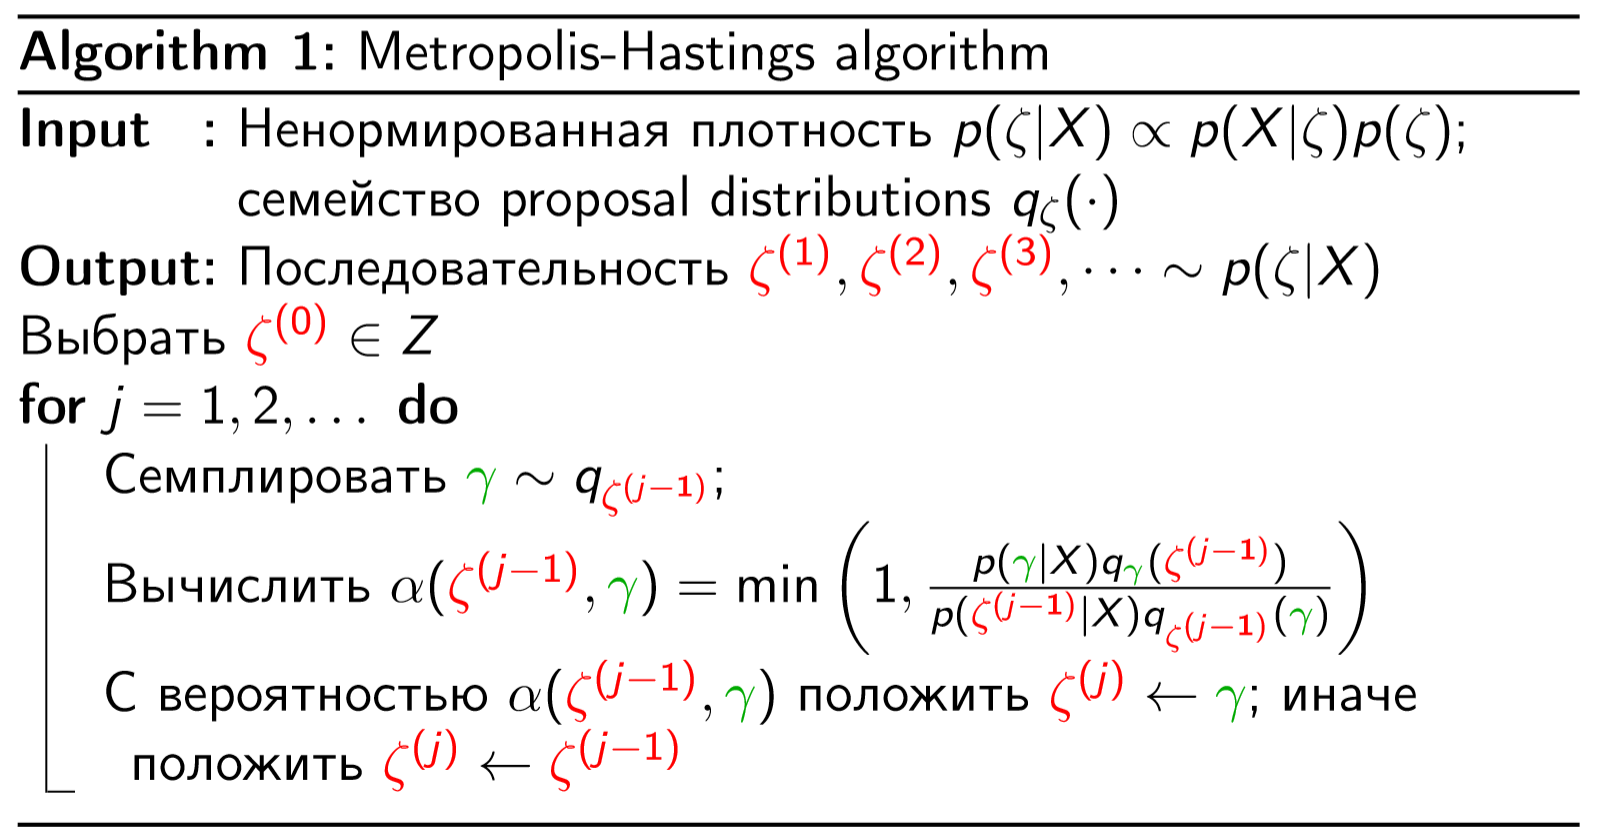
\includegraphics[width=0.8\linewidth]{chapters/petr_mokrov_s1/figs/metr_hast.png}
\end{figure}

\subsection{Application: Particle Physics}

Рассмотрим применение изученных нами потоков на многообразиях в контексте Likelihood-free simulation-based inference для решения задачи из физики частиц

Исследуется симулятор столкновения протонов в LHC. Параметрами модели выступают коэффициенты эффективной теории поля $\zeta \in \bbR^3$, семплируется набор статистик $x \in \bbR^{40}$. Из физики известно, что данные лежат на $14$-D многообразии.

Результаты работы моделей представлены на таблице ниже: 

\begin{figure}[h]
    \centering
    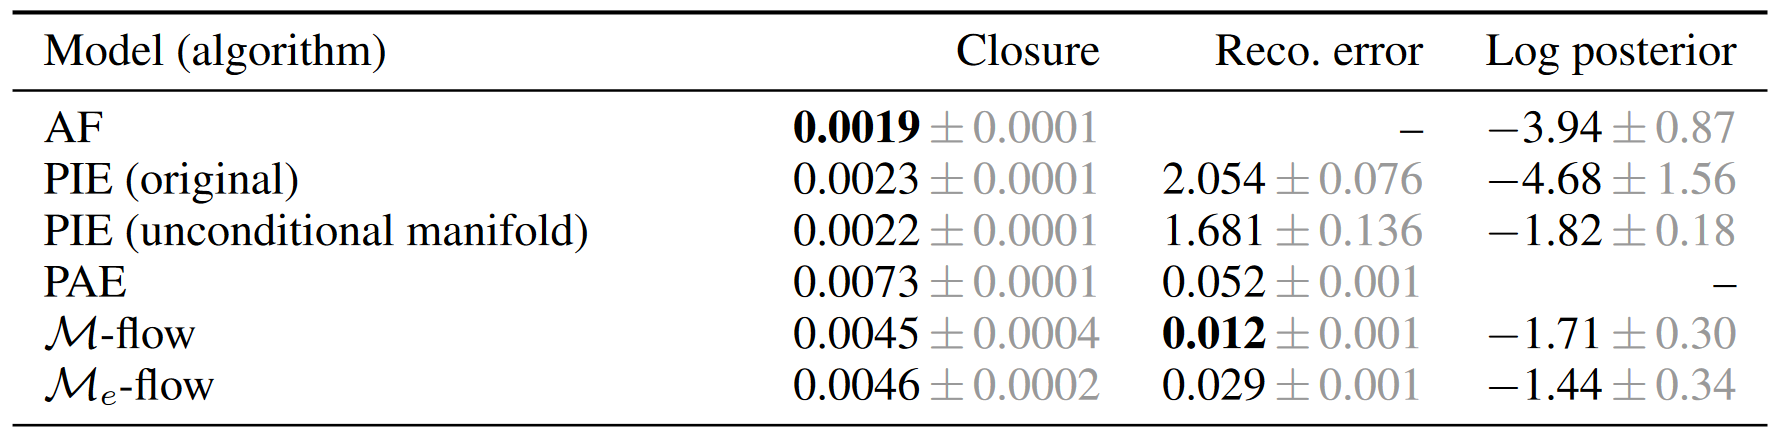
\includegraphics[width=0.9\linewidth]{chapters/petr_mokrov_s1/figs/particle_physics_res.png}
\end{figure}

\sunset{Closure} - тесты корректности генеративной модели; \sunset{Reco. error} - расстояние тестовой выборки до её проекции на выученное многообразие; \sunset{Log posterior} - правдоподобие истинного $\zeta^*$ на posterior KDE, построенного по MCMC.




\section{Questions To Discussion}
\begin{enumerate}
    \item Почему обычные потоки (AF) плохо оценивают плотность при моделировании данных на многообразиях?
    \item Какие вычислительные проблемы возникают у Rectangular flows ($\cM, \cM_e$ - flows) при оценке плотности?
    \item Каким образом можно спроецировать точку на многообразие, моделируемое $\cM$-потоком?
    \item В чём отличие между $\cM$ и $\cM_{e}$ потоками?
    \item Каким образом удаётся избежать сложных вычислений при семплировании из апостериорного распределения на параметрах модели с использованием MCMC в задаче simulation-based inference?
\end{enumerate}